\acrfull{rag} improves \glspl{llm} by integrating real-time data retrieval into the generative process \cite{singh2025}.
Unlike static \glspl{llm} that rely on pre-trained knowledge, \gls{rag} dynamically retrieves relevant external information, improving response accuracy, contextual relevance and updateability \cite{Fan2024, singh2025}.

When a user's query requires information beyond the training data of a \gls{llm}, such as real-time knowledge or unseen facts, the model's response may be outdated or incomplete.
In such cases, standard \glspl{llm} without external retrieval mechanisms struggle to provide accurate answers, as illustrated in the upper part of the Fig.~\ref{fig:rag-no-rag-example}.
Here, the model fails to answer a simple fact-based question about the winner of the 2023 Women's World Cup due to its training data cutoff.
However, with \gls{rag}, as shown in the lower part of the image, the system retrieves relevant information from an external database before generating a response.
This enables the model to produce up-to-date and contextually accurate answers by grounding its output in real-world knowledge.

\begin{figure}[htbp]
    \centering
 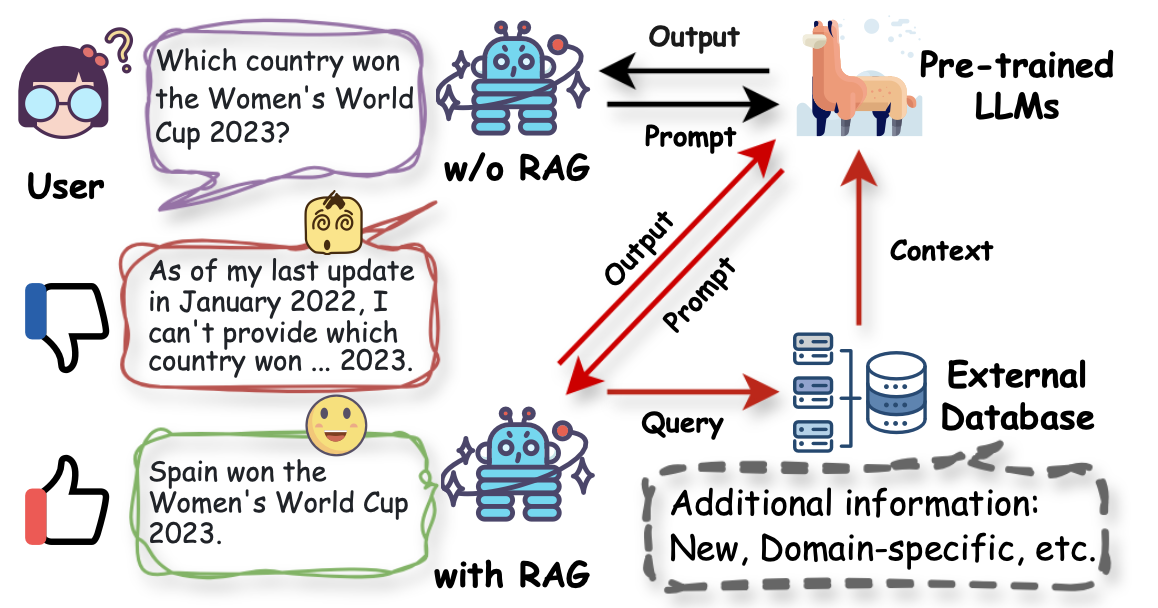
\includegraphics[width=.7\textwidth]{figures/literature-review/rag-no-rag-example.png}
     \rule{35em}{0.5pt}
    \caption{An example of the limitations of \glspl{llm} without retrieval mechanisms (top) and the benefits of \gls{rag} with real-time data retrieval (bottom) (\textcite{Fan2024})}
 \label{fig:rag-no-rag-example}
\end{figure}

Fig.~\ref{fig:rag-components} shows the three main components of \gls{rag}:
\begin{itemize}
    \item \textbf{Retrieval}: queries external sources such as knowledge bases, APIs or vector databases, using dense vector search and advanced transformer-based models to improve accuracy.
	\item \textbf{Augmentation}: processes, extracts and synthesises the retrieved data to align it with the user's query.
	\item \textbf{Generation}: combines the retrieved information with the \gls{llm}'s internal knowledge to produce coherent and contextually relevant answers. 
\end{itemize}
	
\begin{figure}[htbp]
    \centering
 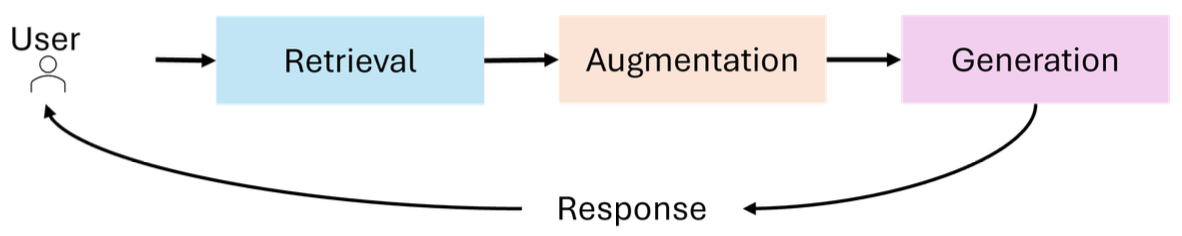
\includegraphics[width=.7\textwidth]{figures/literature-review/RAGcomponents.png}
     \rule{35em}{0.5pt}
    \caption{\gls{rag} components (\textcite{singh2025})}
 \label{fig:rag-components}
\end{figure}

The evolution of \gls{rag} has given rise to several paradigms, each of which refines the interaction between retrieval and generation to improve contextual accuracy, scalability and reasoning capabilities.
From the basic Na\"ive \gls{rag} to the more sophisticated Advanced \gls{rag}, Modular \gls{rag} and Graph\gls{rag}, these approaches have progressively addressed major limitations.
The newest and most powerful paradigm, Agentic \gls{rag}, introduces autonomous agents that dynamically adapt retrieval strategies, optimise workflows and enable complex multi-stage reasoning.
Each paradigm is briefly described in the next subsections.
Table~\ref{table:rag-paradigms-comparison} provides a comparison of the key features, strengths and challenges of these \gls{rag} paradigms.

\subsection*{Na\"ive \gls{rag}}\label{sec:naive-rag}
Na\"ive \gls{rag} is the most fundamental implementation of \gls{rag}, characterized by a straightforward retrieve-read framework \cite{gao_retrieval-augmented_2024}.
It consists of three main steps: indexing, retrieval, and generation \cite{gao_retrieval-augmented_2024,singh2025}.
During indexing, raw data from various sources (e.g., PDFs, Word documents, HTML) is cleaned, segmented into smaller text chunks, and embedded into a vector representation using an embedding model before being stored in a vector database.
When a user poses a query, the system retrieves the most relevant text chunks based on semantic similarity using the same embedding model.
These retrieved chunks are then incorporated into the generation phase, where a \gls{llm} synthesizes a response using both the retrieved information and its internal knowledge.
While Na\"ive \gls{rag} effectively enhances \glspl{llm} by integrating external knowledge, it suffers from several limitations, described as follows.
Retrieval inefficiencies: the retrieved chunks may be irrelevant, misaligned, or miss crucial context, reducing the quality of responses \cite{gao_retrieval-augmented_2024,singh2025}.
Hallucinations: the \gls{llm} may generate content unsupported by retrieved data, leading to factual inaccuracies \cite{gao_retrieval-augmented_2024}.
Redundancy and inconsistency: retrieved information may be overlapping or disjointed, making it challenging to generate coherent answers \cite{gao_retrieval-augmented_2024}.
Limited adaptability: a single retrieval pass based on the original query might not capture sufficient context, restricting performance in complex tasks \cite{gao_retrieval-augmented_2024,singh2025}.
Despite its simplicity, Na\"ive \gls{rag} provided the foundation for more advanced \gls{rag} paradigms, such as Advanced \gls{rag} and Modular \gls{rag}, which introduce retrieval optimization, re-ranking mechanisms, and multi-step reasoning to address these challenges.

\subsection*{Advanced \gls{rag}}\label{sec:advanced-rag}
Advanced \gls{rag} enhances the limitations of Na\"ive \gls{rag} by integrating sophisticated retrieval optimization techniques and semantic understanding to improve information retrieval and generation quality \cite{gao_retrieval-augmented_2024}.
Unlike Na\"ive \gls{rag}, which relies on simple keyword-based retrieval, Advanced \gls{rag} employs \gls{dpr} \cite{Karpukhin2020} and neural ranking algorithms to prioritize relevant information \cite{singh2025}.
It introduces pre-retrieval optimizations such as query expansion, metadata enrichment, and indexing improvements to refine the quality of retrieved data.
Additionally, it implements post-retrieval techniques like context re-ranking, summarization, and adaptive filtering, ensuring that the retrieved information aligns more effectively with the user query before being fed into the language model.
Furthermore, Advanced \gls{rag} supports multi-hop retrieval, allowing the system to retrieve and combine insights from multiple sources to generate well-informed and contextually aware responses.
These enhancements make it more scalable and precise, making it well-suited for knowledge-intensive applications such as scientific research, legal reasoning, and enterprise search solutions.
However, it comes with challenges such as higher computational overhead and latency due to complex retrieval and ranking processes.

\subsection*{Modular \gls{rag}}\label{sec:modular-rag}
Modular \gls{rag} addresses the limitations of Na\"ive and Advanced \gls{rag} by incorporating flexible and composable components, enabling greater adaptability and optimization for specific use cases \cite{gao_retrieval-augmented_2024}.
In contrast to the linear pipeline of traditional \gls{rag}, Modular \gls{rag} enables independent modification and replacement of retrieval, augmentation, and generation modules, making it highly customizable.
According to \cite{singh2025}, key enhancements include hybrid retrieval strategies, where both sparse (e.g., BM25) and dense retrieval \cite{Karpukhin2020} (e.g., \gls{dpr}) techniques are combined for better query matching, and multi-source retrieval, which integrates structured (databases, \glspl{kg}) and unstructured (documents, APIs) sources.
Moreover, modular \gls{rag} introduces new modules like adaptive search, memory, and task-specific adapters, along with new patterns such as iterative retrieval and dynamic module reconfiguration, enhancing flexibility and precision across diverse applications \cite{gao_retrieval-augmented_2024}.
Modular \gls{rag} also supports dynamic query rewriting and multi-step reasoning, allowing iterative refinements to retrieval results.
Its modular design makes it ideal for domain-specific tasks, such as financial analytics and scientific research, where different retrieval and augmentation techniques are needed.
However, this paradigm faces challenges in complex data integration, requiring handling of unstructured, semi-structured, and structured data; system orchestration, demanding precise workflow management across modular components; and component selection and optimization, ensuring individual modules are fine-tuned and effectively integrated for optimal performance.
Fig.~\ref{fig:naive-advanced-modular-rag} illustrates the evolution of the three \gls{rag} paradigms just described, comparing Na\"ive, Advanced and Modular \gls{rag}, highlighting their key components, optimisations and structural differences.
\begin{figure}[htbp]
    \centering
 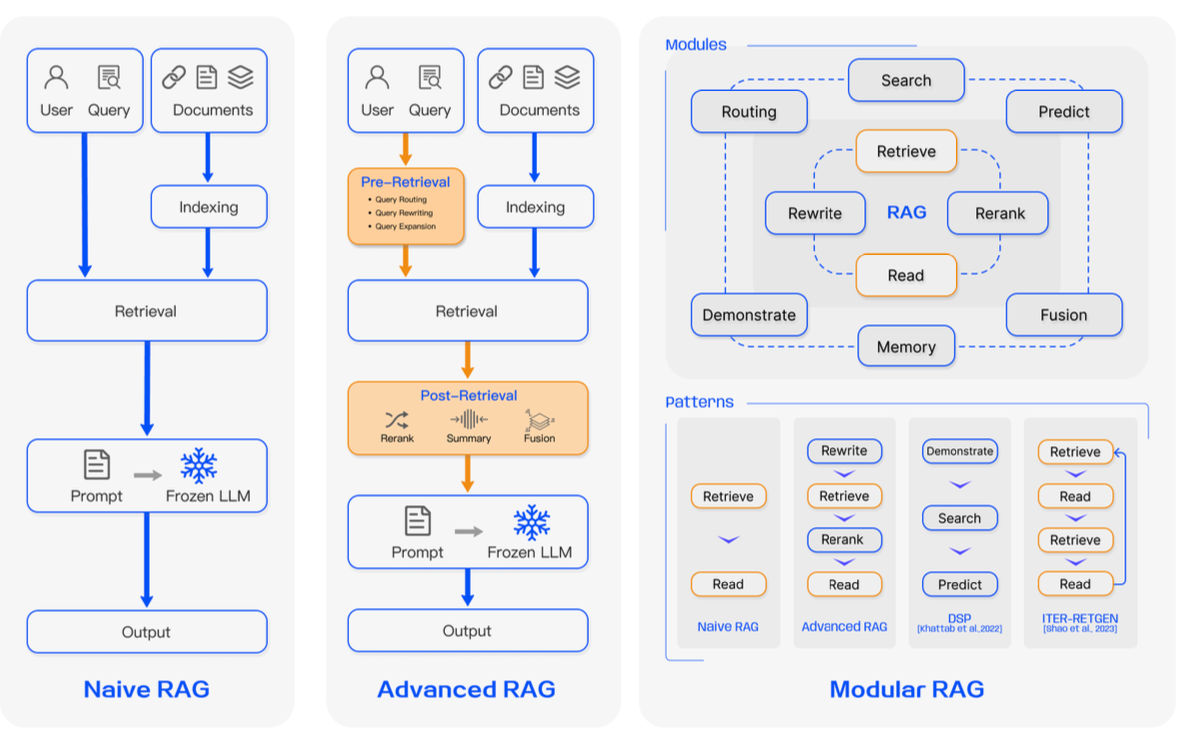
\includegraphics[width=.75\textwidth]{figures/literature-review/naive-advanced-modular-rag.png}
     \rule{35em}{0.5pt}
    \caption{Na\"ive, Advanced and Modular \gls{rag} architectures (\textcite{gao_retrieval-augmented_2024})}
 \label{fig:naive-advanced-modular-rag}
\end{figure}

\subsection*{Graph\gls{rag}}\label{sec:graph-rag}
Graph\gls{rag} is an advanced \gls{rag} framework that leverages structured \glspl{kg}, as illustrated in Fig.~\ref{fig:graph-rag-architecture} , to improve contextual understanding and response generation by \glspl{llm} \cite{peng2024graphragsurvey,singh2025}.
Unlike traditional \gls{rag} approaches that rely solely on retrieving textual information, Graph\gls{rag} incorporates relational knowledge by retrieving structured graph elements, such as nodes, triples, paths, or subgraphs, from a pre-constructed graph database.
This allows for more accurate and context-aware responses, as it captures entity relationships that text-based methods often overlook \cite{singh2025}.
One of the key distinctions between Graph\gls{rag} and standard \gls{rag} is its ability to maintain and utilize explicit structural connections, whereas text-based \gls{rag} primarily depends on similarity-based retrieval from unstructured text corpora.
Graph\gls{rag} thus reduces redundancy and enhances global information retrieval by abstracting and summarizing textual data into a more structured form.
Among its advantages, Graph\gls{rag} enables more precise and comprehensive retrieval, effectively capturing relational knowledge that improves factual consistency and mitigates hallucination.
Additionally, it facilitates query-focused summarization by retrieving subgraphs that include broader contextual information, reducing verbosity in responses.
However, Graph\gls{rag} also presents limitations, including scalability challenges due to the exponential growth of subgraph candidates and the dependency on high-quality, well-structured graph data \cite{singh2025}.
Integrating graph-based retrieval with unstructured retrieval mechanisms adds complexity to implementation, making Graph\gls{rag} more computationally demanding than traditional \gls{rag} approaches \cite{peng2024graphragsurvey,singh2025}.

\begin{figure}[htbp]
    \centering
 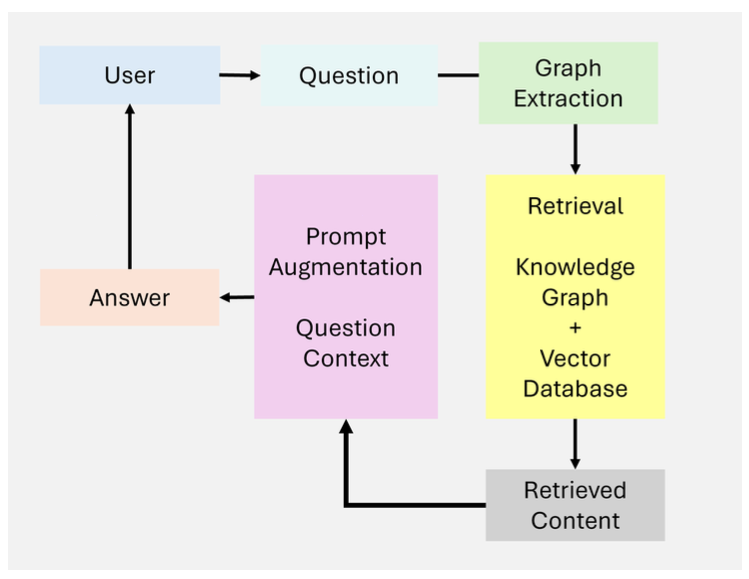
\includegraphics[width=.65\textwidth]{figures/literature-review/graphRAG.png}
     \rule{35em}{0.5pt}
    \caption{Graph\gls{rag} architecture (\textcite{singh2025})}
 \label{fig:graph-rag-architecture}
\end{figure}

\subsection*{Agentic \gls{rag}}\label{sec:agentic-rag}
Agentic\gls{rag} extends traditional \gls{rag} frameworks by integrating autonomous agents that dynamically manage retrieval, reasoning, and response generation workflows \cite{singh2025}.
Unlike standard \gls{rag} systems, which rely on predefined retrieval pipelines, Agentic\gls{rag} incorporates agentic design patterns such as reflection, planning, tool use, and multi-agent collaboration to enable adaptive decision-making and iterative refinement.
These autonomous agents assess query complexity, refine search strategies, and optimize knowledge integration, leading to improved contextual accuracy and scalability.
A key advantage of Agentic\gls{rag} is its ability to manage multi-step reasoning processes, allowing for more precise responses to complex queries.
By dynamically orchestrating workflows, these systems enhance retrieval efficiency and minimize hallucinations by iteratively validating retrieved content.
However, the increased complexity of Agentic\gls{rag} poses challenges, including higher computational overhead and the need for sophisticated coordination mechanisms among multiple agents.
An example of a Multi-Agent Agentic\gls{rag} architecture is shown in Fig.~\ref{fig:multi-agent-agentic-rag}.
Additionally, while it improves adaptability, the unpredictability of agent-driven workflows can introduce variability in response generation.
Despite these challenges, Agentic\gls{rag} is particularly well-suited for domains requiring dynamic adaptability, such as financial analytics, healthcare diagnostics, and legal research, where multi-agent collaboration and iterative refinement enhance the reliability of \gls{ai}-generated insights \cite{singh2025}.

\begin{figure}[htbp]
    \centering
 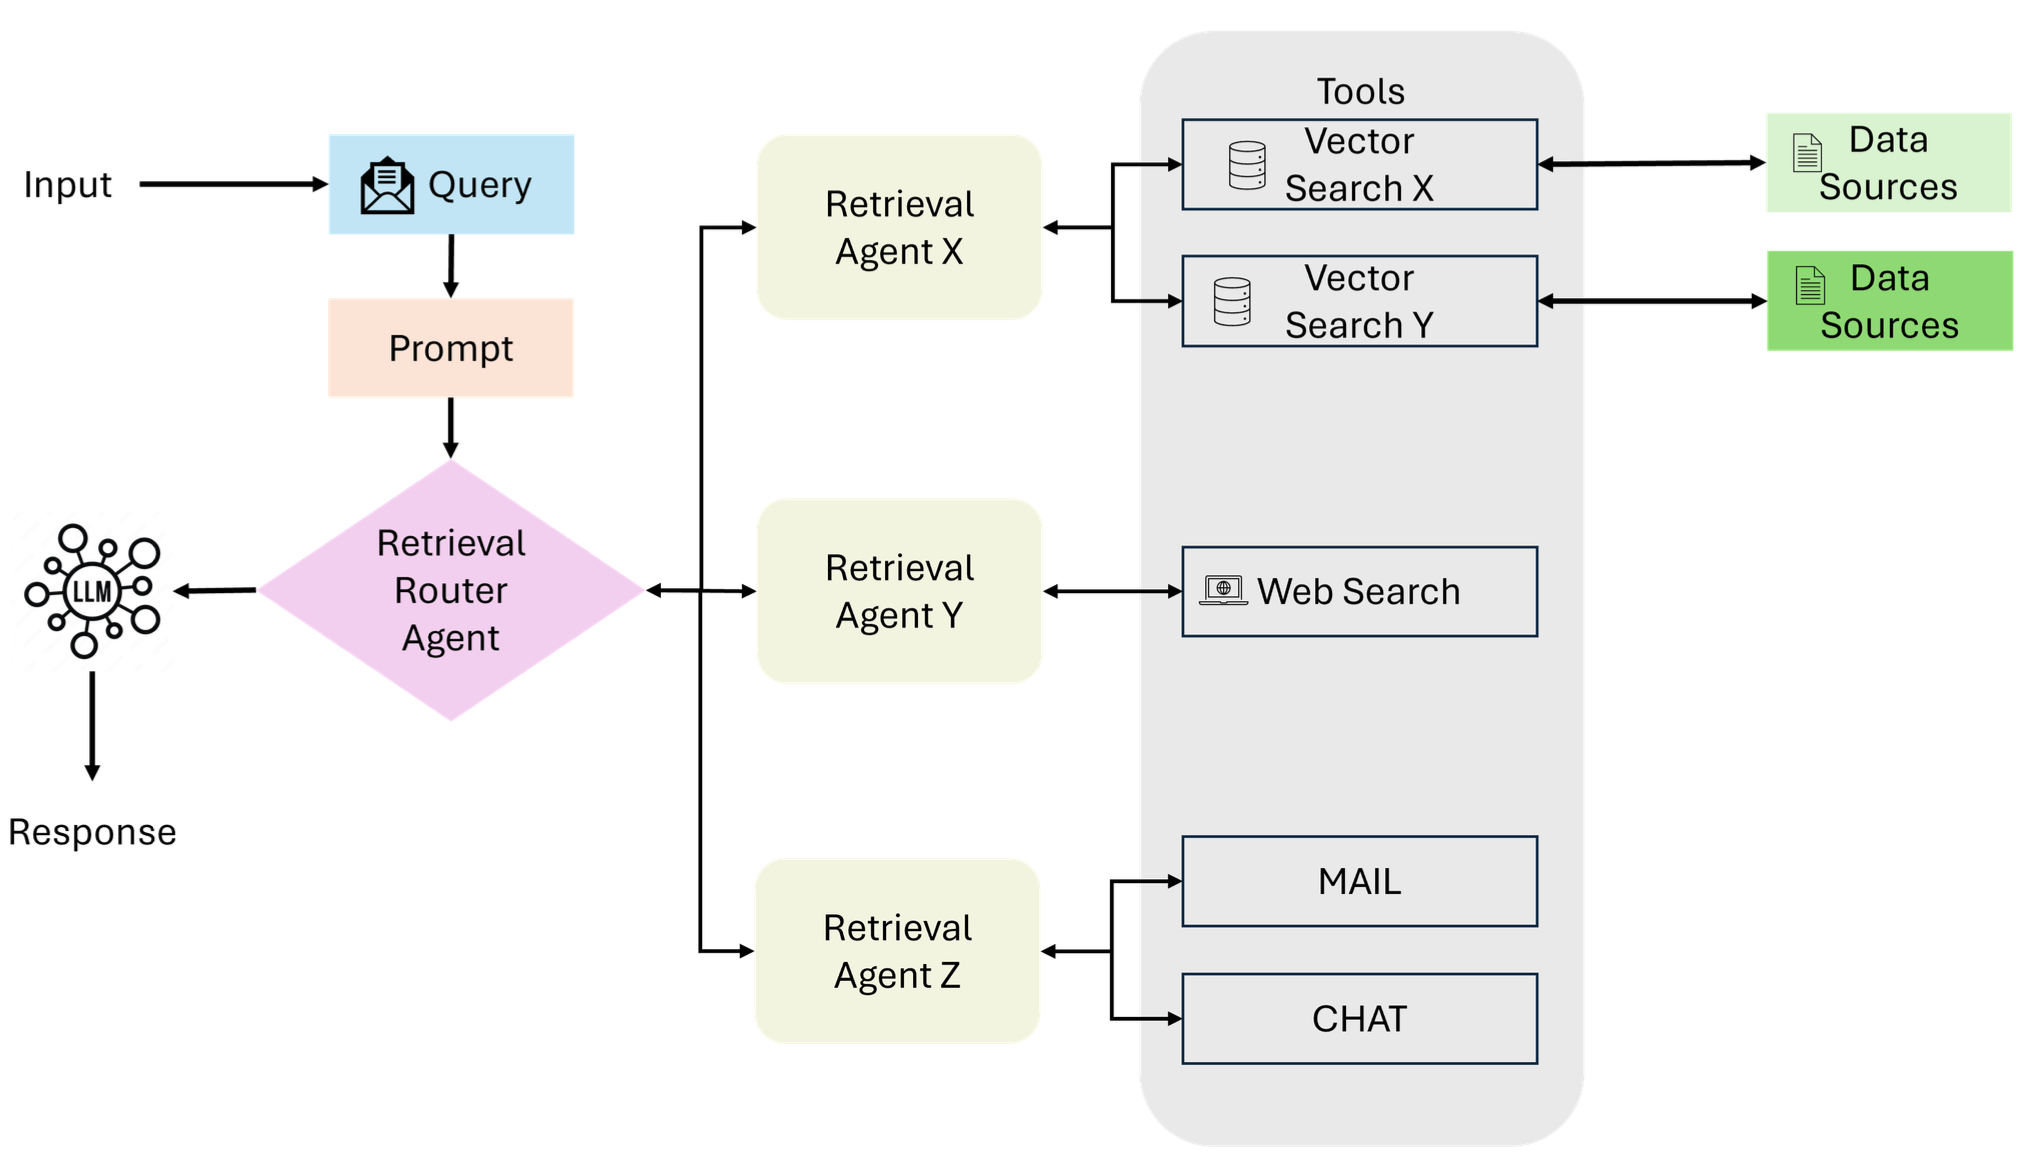
\includegraphics[width=.8\textwidth]{figures/literature-review/multi-agent-agentic-rag.png}
     \rule{35em}{0.5pt}
    \caption{Multi-Agent Agentic\gls{rag} architecture (\textcite{singh2025})}
 \label{fig:multi-agent-agentic-rag}
\end{figure}

\begin{table}[htbp]
    \centering
    \scriptsize
    \begin{tabularx}{\textwidth}{|>{\centering\arraybackslash}p{1.5cm}|X|X|X|}
      \hline
      \textbf{\gls{rag} Paradigm} & \textbf{Key Features} & \textbf{Strengths} & \textbf{Challenges}\\
      \hline
          \begin{center}
            Na\"ive
          \end{center} & \begin{itemize}[nosep, left=0pt]
        \item Keyword-based retrieval (e.g., TF-IDF, BM25)
      \end{itemize} & \begin{itemize}[nosep, left=0pt]
        \item Simple and easy to implement
        \item Suitable for fact-based queries
      \end{itemize}& \begin{itemize}[nosep, left=0pt]
        \item Retrieval inefficiency
        \item Hallucinations
        \item Redundancy and inconsistency
        \item Limited adaptability
      \end{itemize}\\
      \hline
      \begin{center}
      Advanced
      \end{center} & \begin{itemize}[nosep, left=0pt]
        \item Dense retrieval models (e.g., DPR)
        \item Neural ranking and re-ranking
        \item Multi-hop retrieval
      \end{itemize} & \begin{itemize}[nosep, left=0pt]
        \item High precision retrieval
        \item Improved contextual relevance
      \end{itemize} & \begin{itemize}[nosep, left=0pt]
        \item Higher computational overhead
        \item Latency
      \end{itemize}\\
      \hline
      \begin{center}
        Modular
      \end{center} & \begin{itemize}[nosep, left=0pt]
        \item Hybrid retrieval (sparse and dense)
        \item Tool and API integration
        \item Composable, domain-specific pipelines
      \end{itemize} & \begin{itemize}[nosep, left=0pt]
        \item High flexibility and customization
        \item Suitable for diverse applications
        \item Scalable
      \end{itemize} & \begin{itemize}[nosep, left=0pt]
        \item Complex data integration
        \item System orchestration and workflow management
        \item Component selection and optimization
        \item Maintenance
      \end{itemize}\\
      \hline
      \begin{center}
        Graph
      \end{center} & \begin{itemize}[nosep, left=0pt]
        \item Integration of graph-based structures
        \item Multi-hop reasoning
        \item Contextual enrichment via nodes
      \end{itemize}& \begin{itemize}[nosep, left=0pt]
        \item Relational reasoning capabilities
        \item Mitigates hallucinations
        \item Ideal for structured data tasks
      \end{itemize}& \begin{itemize}[nosep, left=0pt]
        \item Scalability challenges
        \item Dependency on high-quality graph data
        \item Complexity of integration
      \end{itemize}\\
      \hline
      \begin{center}
        Agentic
      \end{center} & \begin{itemize}[nosep, left=0pt]
        \item Autonomous agents
        \item Dynamic decision-making
        \item Iterative refinement and workflow optimization
      \end{itemize}& \begin{itemize}[nosep, left=0pt]
        \item Adaptable to real-time changes
        \item Scalable for multi-domain tasks
        \item High accuracy
      \end{itemize} & \begin{itemize}[nosep, left=0pt]
        \item Coordination complexity
        \item Computational overhead
        \item Scalability challenges
      \end{itemize}\\
      \hline
    \end{tabularx}
    \caption{\gls{rag} paradigms comparison adapted from \textcite{singh2025} and extended by the author}
    \label{table:rag-paradigms-comparison}
  \end{table}